\documentclass[10.5pt]{article} 
\usepackage[utf8]{inputenc}   
\usepackage[english]{babel}  
\usepackage{amsmath}   
\usepackage{ amssymb }
\usepackage{amsfonts}         
\usepackage{geometry}          
\usepackage{graphicx}
\usepackage{float}
\usepackage{xcolor}
\usepackage{ulem}
\usepackage{tcolorbox}
\usepackage{cancel} 
\usepackage{tikz}
\usepackage{framed}
\usepackage{mdframed}
\usepackage{cite}
\usepackage{hyperref}

\usepackage{parskip} 
\setlength{\parskip}{8pt plus 2pt minus 1pt} 
\setlength{\parindent}{0pt} 

\usepackage{xparse}

\geometry{a4paper, margin=1in} 

\title{\textbf{Projects IV. Graphics Programming, Immersive Systems and Video Games. Block 2.}}
\author{César Vidal Fernández}
\date{November 12, 2026}

\definecolor{ejercicio}{RGB}{59, 88, 102}
\definecolor{explicacion}{rgb}{0.008, 0.161, 0.098}

\newcommand{\tachareq}[1]{\textcolor{black}{\cancel{#1}}}
\newcommand{\dvt}[1]{\;\mathrm{d}#1}
\newcommand{\separation}{\vspace{10px} \rule{\textwidth}{0.6pt} \par}
\newcommand{\lagrangian}{\mathcal{L}}
\newcommand{\ejercicio}[1]{\color{ejercicio}\textbf{\uline{#1}}\color{black}}
\newcommand{\explicacion}[1]{\color{explicacion}\textit{#1}\color{black}}

\newenvironment{sideline}
{\begin{mdframed}[
		linewidth=1pt,
		topline=false,
		bottomline=false,
		rightline=false,
		leftline=true,
		leftmargin=0cm,
		rightmargin=0cm,
		innertopmargin=0.5cm,
		innerbottommargin=0.5cm
		]}
	{\end{mdframed}}

\begin{document}
	
	\renewcommand{\contentsname}{Contents.}
	
	\maketitle	
	\newpage
	
	\tableofcontents
	\newpage
	
	\section{Introduction and Scope of the Project.}
	
	As set out in the previous block, the simulation will consist of an audiovisual representation of an aircraft breaking the sound barrier in an immersive, interactive environment running in real time.
	
	This allows the complex equations of fluid mechanics (such as the compressible Navier--Stokes equations) to be reduced significantly, either by considering specific cases or by introducing simplifications, which are detailed in the following section. 
	
	The fundamental aim of the model is to recreate, in real time, the kinematics of the wavefronts and the acoustics of moving sources undergoing uniform acceleration.
	
	The aircraft under study is the \textit{Concorde}, a passenger airliner in commercial service between 1976 and 2003, jointly funded by the British and French governments. 
	
	\begin{figure}[H]
		\centering
		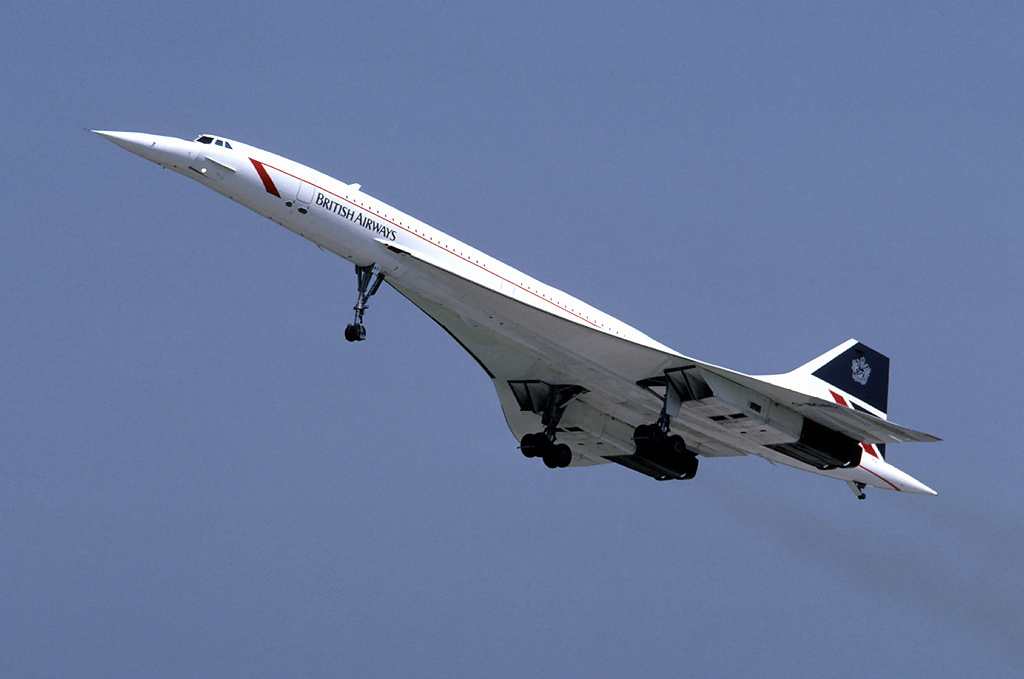
\includegraphics[width=0.6\textwidth]{imgs/concorde.jpg}
		\caption{A British Airways Concorde. Source: \cite{concorde_wiki}}
	\end{figure}
	
	\subsection{Terminology.}
	
	\begin{itemize}
		\item Mach: a unit of speed expressed relative to the speed of sound in the medium through which the moving body travels. At sea level, 1 Mach = 343 m/s. This is purely a reference value; for the purposes of this study, it is computed as a variable that depends on altitude. 
		
		\item Wave: in the context of audio synthesis, a wave is the basic building block, and it can take different shapes depending on how we want it to behave over time. This document deals mainly with the N-wave, which is explained in simple terms later on, and with random noise, whose waveform is, by definition, random. 
		
		\begin{figure}[H]
			\centering
			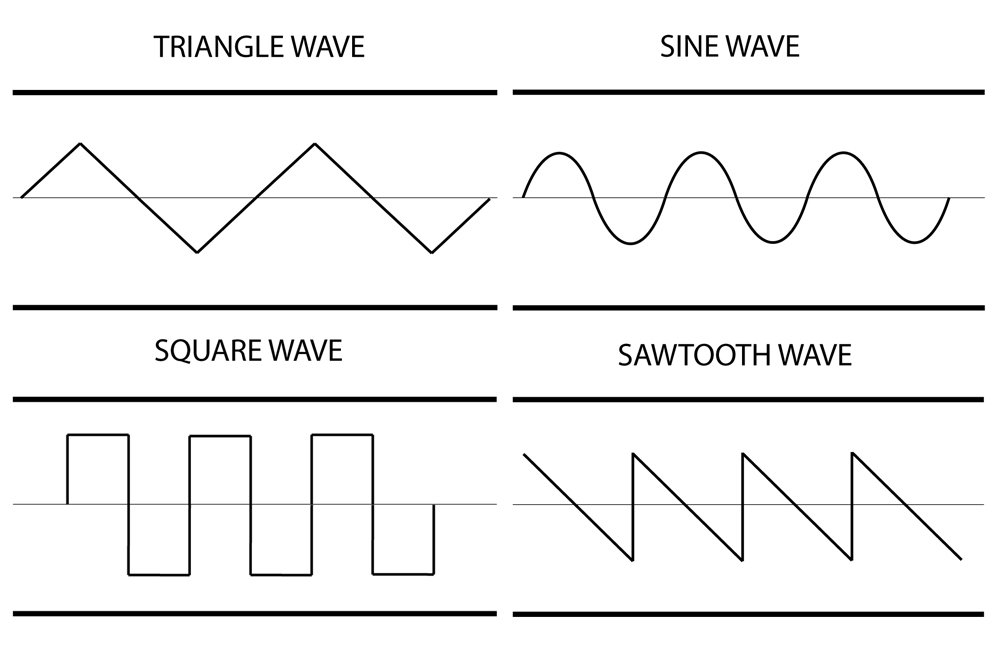
\includegraphics[width=0.5\textwidth]{imgs/waveforms.jpg}
			\caption{Sine, square, triangle, and sawtooth waveforms. Source: \cite{wave_forms}}
		\end{figure}
	\end{itemize}
	
	\newpage 
	\section{Governing Equations.}
	
	Three clearly distinct conceptual and mathematical blocks are identified as governing the behavior of the system in real time.
	
	\subsection{Aircraft Motion (1D Kinematics and Mach Number).}
	
	The phenomenon of interest occurs at high speed. For the chosen aircraft model, the \textit{Concorde}, the acceleration towards the supersonic regime began at high altitude. The phases of the flight are outlined below in order to fully understand how the aircraft operated \cite{912161}.
	
	\begin{enumerate}
		\item Initial subsonic phase: the aircraft takes off conventionally and, owing to noise-pollution regulations near populated areas, remains subsonic until it reaches an altitude of between 8,500 and 9,100 meters, at a speed of Mach 0.95. 
		
		\item \textbf{Acceleration and breaking the sound barrier}: the afterburners are lit, the vertical angle of attack is reduced in order to begin a more gradual climb, and the speed is progressively increased until Mach 2 is reached at 15,200 meters.
		
		\item Cruise: cruising takes place at the altitude and speed reached at the end of the previous phase. 
	\end{enumerate}
	
	To simplify the study and work in a single dimension (analogous to an inclined-plane problem), the following assumptions and simplifications are made:
	
	\begin{itemize}
		\item A rotated coordinate system is defined, in which the aircraft's climb trajectory runs along an axis inclined at an angle $\theta$ to the horizontal.
		
		\item The acceleration is taken to be constant and the climb trajectory to be perfectly linear.
	\end{itemize}
	
	The motion of the aircraft is modeled in terms of the distance $s(t)$ travelled along the climb ramp, which undergoes uniformly accelerated rectilinear motion:
	
	\begin{equation*}
		s(t) = s_0 + v_0 \cdot t + \frac{1}{2} \cdot a \cdot t^2
	\end{equation*}
	
	Projecting this onto the two-dimensional $(x, y)$ plane by means of the geometric components of the inclined plane, the position vector of the aircraft as a function of time is:
	
	\begin{equation*}
		\vec{r}_{\text{aircraft}}(t) = \left( x_0 + s(t)\cos\theta, \, y_0 + s(t)\sin\theta \right)
	\end{equation*}
	
	Taking the time origin $t_0 = 0$ at the start of the acceleration phase, with initial velocity $v_0$ along the ramp, the instantaneous velocity vector of the source in 2D is:
	
	\begin{equation*}
		\vec{v}_{\text{aircraft}}(t) = (a \cdot t + v_0)\cos\theta \, \hat{i} + (a \cdot t + v_0)\sin\theta \, \hat{j}
	\end{equation*}
	
	Its scalar magnitude along the direction of climb is:
	
	\begin{equation*}
		v_{\text{aircraft}}(t) = \|\vec{v}_{\text{aircraft}}(t)\| = a \cdot t + v_0
	\end{equation*}
	
	The speed of sound ($c$) in an ideal gas depends on the local temperature of the medium ($T$):
	
	\begin{equation*}
		c(T) = \sqrt{\gamma \cdot R \cdot T}
	\end{equation*}
	
	where $\gamma = 1.4$ is the adiabatic index of air and $R = 287\text{ J/(kg}\cdot\text{K)}$ is the specific gas constant of air. Evaluating the temperature from the reference atmospheric model at the corresponding altitude along the ramp, the flight regime is characterized by the \textbf{instantaneous Mach number}:
	
	\begin{equation*}
		M(t) = \frac{v_{\text{aircraft}}(t)}{c(T)}
	\end{equation*}
	
	\subsection{Visual Model: Wavefront Propagation and Caustics.}
	
	Rather than solving for the kinematic pressure field of the air, the real-time visual representation is based on Huygens' principle. The surface of the aircraft acts as a continuous emitter of spherical sound disturbances, one emitted at each instant $t_e$.
	
	The center of each sphere is the position the aircraft occupied at the moment of emission. The superposition of these spheres gives rise to the Mach cone. 
	
	\begin{figure}[H]
		\centering
		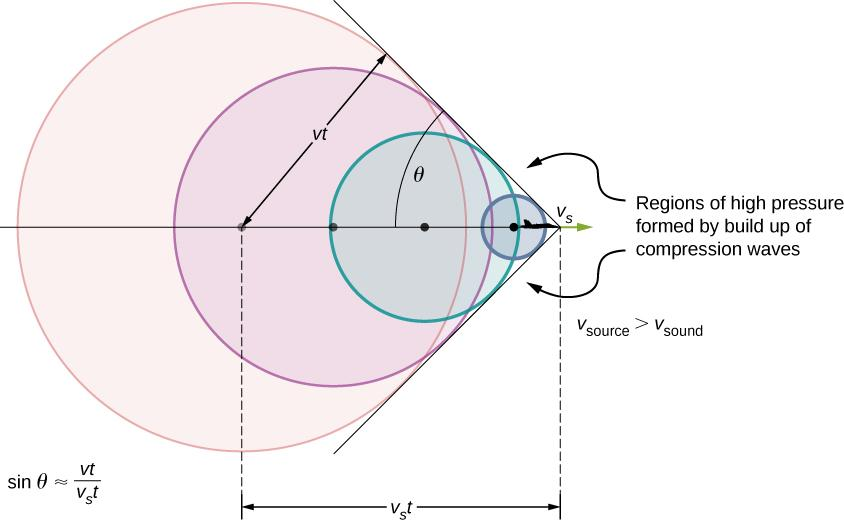
\includegraphics[width=0.6\textwidth]{imgs/rotura.jpg}
		\caption{Mach cone. Source: \cite{shockwaves}}
	\end{figure}
	
	The radius $R$ of the wavefront emitted at instant $t_e$, evaluated at the current time $t$, is given by:
	
	\begin{equation*}
		R(t, t_e) = c \cdot (t - t_e) \qquad \text{for } t \ge t_e
	\end{equation*}
	
	The center of this wavefront is located at $x_{\text{emission}} = x_{\text{aircraft}}(t_e)$. The accumulation, or superposition, of these spherical fronts produces the visual envelope of the shock wave. When $M(t) > 1$, the instantaneous Mach cone angle $\mu(t)$ satisfies:
	
	\begin{equation*}
		\sin(\mu(t)) = \frac{1}{M(t)}
	\end{equation*}
	
	Since the source is accelerating ($a > 0$), the envelope of the wavefronts acquires a characteristic curvature (a caustic), marking the visible boundary of the pressure discontinuity in the atmosphere.
	
	In practical terms, the Mach spheres will be assigned an opacity that depends on their radius, so as to give visual priority to the most recently generated ones.
	
	\subsection{Acoustic Model: Retarded Time and Dynamic Doppler Effect.}
	
	For an observer located at position $\mathbf{r}_{\text{obs}}$, the sound perceived at instant $t$ originates from the position the aircraft occupied at the retarded emission instant $t_e$. This instant is the solution of the retarded-time equation:
	
	\begin{equation*}
		t - t_e = \frac{\|\mathbf{r}_{\text{obs}} - \mathbf{r}_{\text{aircraft}}(t_e)\|}{c}
	\end{equation*}
	
	The change in frequency perceived by the observer due to the relative Doppler effect with an accelerating source is given by:
	
	\begin{equation*}
		f_{\text{obs}}(t) = \frac{f_0}{1 - \dfrac{\mathbf{v}_{\text{aircraft}}(t_e) \cdot \mathbf{n}(t_e)}{c}}
	\end{equation*}
	
	where $\mathbf{n}(t_e) = \frac{\mathbf{r}_{\text{obs}} - \mathbf{r}_{\text{aircraft}}(t_e)}{\|\mathbf{r}_{\text{obs}} - \mathbf{r}_{\text{aircraft}}(t_e)\|}$ is the unit line-of-sight vector from the emission position towards the observer.
	
	At the exact moment the envelope of the shock wave passes through the observer's position ($\mathbf{v}_{\text{aircraft}} \cdot \mathbf{n} = c$), the denominator theoretically vanishes. This results in the simultaneous arrival of many accumulated wavefronts and produces the acoustic overpressure signature known as the \textit{sonic boom}, or N-wave signature.
	
	Although the instant at which the phenomenon reaches the listener depends entirely on the reference frame, the perceived intensity does not, since there is a real attenuation directly related to the time and distance travelled by the sound waves.
	
	\begin{equation*}
		\text{Gain} = \frac{1}{\|\mathbf{r}_{\text{obs}} - \mathbf{r}_{\text{aircraft}}(t_e)\|}
	\end{equation*}
	
	
	\subsubsection{Sound Generation.}
	
	Two main sound sources are distinguished, both of which will have to be modeled from scratch. It has been decided not to use audio files and instead to synthesize the sounds with numerical algorithms, adding a further layer of complexity and customization to the overall sound of the simulation.
	
	\begin{itemize}
		\item \textbf{Base noise generation (turbine)}: a constant layer present for as long as the aircraft is in flight. The signal is computed anew in every frame.
		\begin{enumerate}
			\item \uline{Generation of the base sound}: the starting point is a stream of white noise, that is, a random signal. This sound will be shaped with equalizers and band-pass filters to give it the required character. 
			
			\textit{White noise on its own, as we know it, is the hiss characteristic of television static. We need to be able to shape specific parameters precisely in order to turn it into the characteristic roar of a jet turbine.}
			
			For practical purposes, we should focus on the resonant frequencies of the turbine's exhaust gases, which typically lie around 200, 800, and 2,500 Hz. This noise can be multiplied by a slightly randomized low-frequency signal, which will give it an organic feel. These parameters will be fixed at later stages of the project and will require some experimentation.
			
			\item \uline{Application of the Doppler effect} according to the retarded time: taking into account the position of the observer relative to the aircraft, the delay due to the finite speed of sound must be accounted for. As an observable result, the pitch will rise as the aircraft approaches and then drop abruptly once it has passed. 
			
			
		\end{enumerate}
		
		\item \textbf{The sonic boom}: an isolated event, beginning at the moment the shock wave reaches the observer. 
		
		\begin{enumerate}
			\item Mathematical construction of the wave (N-wave): as discussed in previous sections, the blast wave has two very specific moments: the instant of impact with the nose and that of impact with the tail.
			
			For this reason, an N-shaped pulse is chosen, that is, one with two moments of peak loudness, at the beginning and at the end, and with a strong emphasis around 30--60 Hz. The aim is to add plenty of sub-bass, with a very pronounced \textit{decay}.
			
			\item Atmospheric crackle: after the bang, micro-vibrations and an abrupt, very high-frequency noise are produced.
			
			\item Reverberation: this sound does not fade away instantly; owing to its high acoustic power, it is reflected by the ground and by the layers of the atmosphere, producing an echo similar to the one heard in a cave or in a very large room. It will be modeled by convolution, with a suitable temporal length, estimated at between 2 and 3 seconds. 
			
		\end{enumerate}
	\end{itemize}
	
	\newpage
	
	\section{Initial and Boundary Conditions.}
	
	The simulation begins at the end of the Concorde's initial climb phase, just before the acceleration towards the supersonic regime starts. The reference initial altitude is 8,500 meters and the corresponding speed is Mach 0.95, in line with the operational characteristics described above.
	
	From this initial state, the aircraft begins a phase of uniform acceleration along an ascending trajectory. The initial conditions of the system are set out below, together with the geometric and physical constraints that delimit the behavior of the simulation.
	
	\subsection{Initial Conditions.}
	
	The initial state of the aircraft is determined by its position, velocity, and acceleration. At the initial instant $t_0=0$, the following conditions are established:
	
	\begin{itemize}
		
		\item \textbf{Initial position and altitude:} the initial altitude is set to $h_0=8500$ meters. The initial horizontal position $x_0$ is used to place the aircraft within the simulation's coordinate system.
		
		\item \textbf{Initial velocity:} this corresponds to the flight regime reached at the end of the initial climb phase. An initial Mach number of $M_0=0.95$ is set, from which the velocity is computed:
		\begin{equation*}
			v_0 = M_0 \cdot c(T_0)
		\end{equation*}
		
		\item \textbf{Atmospheric temperature:} this is determined from the reference air temperature at the initial altitude of 8,500 meters. This value makes it possible to compute the local speed of sound using the expression defined above:
		\begin{equation*}
			c(T_0) = \sqrt{\gamma R T_0}
		\end{equation*}
		
		\item \textbf{Acceleration:} this is taken to be constant throughout the simulation interval. A default reference value corresponding to the Concorde's acceleration phase is used, although this parameter can be modified in order to study different kinematic behaviors.
		
		\item \textbf{Trajectory inclination:} this is defined by the angle $\theta$ to the horizontal. Its default value reproduces the characteristic climb gradient of the flight phase under study, and it can likewise be modified as a simulation parameter.
		
		\item \textbf{Observer position:} this is defined by a position vector $\mathbf{r}_{obs}$, tied to the position of the camera. Two configurations are considered: a camera attached to the aircraft, which allows the phenomenon to be observed from an elevated position relative to it, and a free camera, whose movement can be controlled independently of the aircraft's trajectory.
		
		Although the kinematics of the aircraft are restricted to a vertical climb plane (2D), the system is formulated and solved in a three-dimensional (3D) environment. This allows the observer to be placed at any position in space.
		
	\end{itemize}
	
	In this way, the simulation makes it possible to study the transition from the subsonic to the supersonic regime, and to vary certain physical and geometric parameters in order to observe their influence on the formation of the shock wave.
	
	\subsection{Boundary Conditions.}
	
	Since the project does not aim to solve the compressible Navier--Stokes equations directly, but rather to represent the geometric propagation of acoustic disturbances, no conventional hydrodynamic boundary conditions are imposed. Instead, the following constraints are established to delimit the behavior of the model:
	
	\begin{itemize}
		
		\item \textbf{Aircraft trajectory:} the motion is restricted to a rectilinear trajectory defined by the climb angle $\theta$. Throughout the simulation interval, the direction of motion remains constant and the acceleration is assumed to be uniform.
		
		\item \textbf{Propagation medium:} air is treated as a homogeneous, isotropic medium at rest relative to the reference frame. Acoustic disturbances propagate radially from their point of emission, at a speed determined by the local atmospheric conditions.
		
		\item \textbf{Wavefront propagation:} each disturbance emitted by the aircraft propagates from the position the source occupied at the instant of emission. In the two-dimensional model, the wavefronts are represented by circles whose radius grows with the time elapsed since emission.
		
		\item \textbf{Observer position:} no fixed spatial position is assigned to the observer. Its location depends on the selected camera configuration, which can either remain attached to the aircraft or move freely within the simulation environment. This position determines the computation of the reception time and of the Doppler effect.
		
		\item \textbf{Spatial domain:} the visual representation is limited to the visible area of the scene and the camera's field of view. Wavefronts that leave the rendering domain are no longer displayed, although their physical propagation is not considered to be interrupted.
		
		\item \textbf{Temporal domain:} the simulation runs over a finite interval, continuously updating the kinematic state of the aircraft, the propagation of the wavefronts, and the corresponding acoustic signals.
		
	\end{itemize}
	
	These conditions establish a controlled scenario in which to study the formation and propagation of the shock-wave envelope, as well as its visual and acoustic perception from different positions within the immersive environment.
	
	\newpage 
	
	\section{Numerical Method and Discretization.}
	
	\subsection{Time Discretization.}
	
	The simulation runs in real time. Although the motion under study is naturally continuous, it must be analyzed discretely on a computer.
	
	A computation time step of $\frac{1}{120}$ s and a rendering time step of $\frac{1}{60}$ s are used, the latter being equivalent to 60 fps. This means that for every two simulation steps, one frame is drawn. 
	
	At more advanced stages of the project, the implementation of a \textit{double buffering} system will be considered, together with adjusting these parameters on the basis of performance metrics. 
	
	\subsection{Trajectory Computation.}
	
	Since the analytical solution of the motion is available, it has been decided to evaluate it directly rather than resort to numerical integration methods such as Euler's:
	\begin{equation*}
		s(t) = s_0 + v_0 \cdot t + \frac{1}{2} \cdot a \cdot t^2
	\end{equation*} 
	
	From it, the position and velocity components can be obtained.
	
	\subsection{Discretization of the Wave Sources.}
	
	The aircraft emits disturbances continuously, but our representation cannot be infinite.
	We require a minimum of 10 wavefronts per time step. This is equivalent to $\Delta t_e = \frac{\Delta t}{10} = \frac{1}{120 \cdot 10} = \frac{1}{1200}$ s, that is, 1200 Hz. Each wavefront is computed at a position obtained by subdividing the interval between the current position and the next.
	
	For each of these positions, the radius at the simulated time must be computed:
	\begin{equation*}
		R_k (t) = c(t - t_{e, k})
	\end{equation*}
	
	Wavefronts outside the rendering area are discarded. 
	
	\subsection{Solving for the Retarded Time.}
	
	We must solve:
	
	\begin{equation*}
		t - t_e = \frac{\|\mathbf{r}_{\text{obs}}(t) - \mathbf{r}_{\text{aircraft}}(t_e)\|}{c}
	\end{equation*}
	
	In this case, direct substitution is not possible, since the unknown $t_e$ appears on both sides of the equation. We will resort to a numerical root-finding method (bisection or Newton--Raphson). The performance of both will be evaluated at more advanced stages of the project, at which point a decision will be made as to which to use. 
	
	Special attention must be paid to the choice of initial guess. In the supersonic regime, several solutions may exist for the same reception instant.
	
	\subsection{Audio Discretization and Generation.}
	
	For audio computation, a completely different scale is established from that of the graphical and computational simulation; a smooth representation with a sense of continuity requires a much larger number of samples per second. As a standard reference, we will use a sampling rate of 44,100 Hz:
	\begin{equation*}
		\Delta t_s = \frac{1}{44100} \approx 22.68\ \mu\text{s}
	\end{equation*}
	
	With a block size of 256 samples, we will need to process information every:
	\begin{equation*}
		T_b = \frac{256}{44100} \approx 5.80\ \text{ms} \Rightarrow \text{172 blocks per second.}
	\end{equation*}
	
	\subsubsection{White Noise Generation.}
	
	White noise can be generated from a Gaussian distribution:
	\begin{equation*}
		x[n] \sim \mathcal{N}(0, \sigma ^2)
	\end{equation*}
	
	Special attention must be paid to clipping. As an additional refinement, state tracking could be introduced in the generator so that the signal is not completely reset at every processing block.
	
	\subsubsection{Filter Application.}
	
	Digital filters can be applied to the signal obtained above. The aim is to adjust some of the parameters of the tone so that it can be shaped at will. As mentioned earlier:
	
	\begin{itemize}
		\item Frequency bands and equalization to change the character of the sound.
		\item Amplitude modulation to prevent the sound from remaining static.
	\end{itemize}
	
	\begin{equation*}
		y[n] = H \cdot { x[n]} \qquad \rightarrow \text{H = filtering system}
	\end{equation*}
	
	\subsubsection{Frequency Modification via the Doppler Effect.}
	
	White noise, unlike other sounds such as that of a musical instrument, has no fundamental frequency\footnote{The fundamental frequency is the lowest frequency at which a periodic wave vibrates.}. This means we cannot simply modify its frequency parameter to obtain the desired effect. 
	
	Several solutions can be considered for this problem. In practice, both should be assessed, but the second has a more interesting physical basis and, where possible, is the one that should ultimately be applied:
	
	\begin{enumerate}
		\item Generate a new sound for each aircraft speed. The major drawback is that a very large number of sounds would have to be created for the sense of the aircraft approaching and receding to be sufficiently continuous and realistic.
		
		\item Work with the audio playback speed. A specific frequency cannot be changed, owing to the limitations discussed above, but the overall frequency spectrum can be shifted by speeding up and slowing down playback.
		
		\begin{equation*}
			f_{\text{out}} = k \cdot f_{\text{original}}
		\end{equation*}
		
		The choice of the factor $k$ is not arbitrary; it can be obtained from the relative velocity between the Concorde and the listener:
		% TODO: review this formula. t_e appears multiplying v_s and cos(alpha); the usual form would be k = c / (c - v_s cos(alpha)).
		\begin{equation*}
			k(t) = \frac{c}{c - v_s \cdot t_e \cdot \cos \alpha}
		\end{equation*}
		
		As currently formulated, this solution suffers from the same problem as the previous one: jumps between blocks. Linear interpolation between blocks is proposed.
		
		\textit{To illustrate this, if the aircraft is moving away from us at high speed, we may obtain two very different factors $k$ for two consecutive blocks ($k_0 = 1.0$, $k_1 = 1.1$). This would produce jumps in how we perceive the simulation, detracting considerably from the realism and rigor we aim for.}
		
		\begin{align*}
			k_i &= k_{\text{prev}} + \lambda_i \left(k_{\text{new}} - k_{\text{prev}}\right) \\
			&\Rightarrow \text{$\lambda_i$ varies progressively between 0 and 1.} \\
			&\Rightarrow i = \text{a specific sample within an audio block.}
		\end{align*}
	\end{enumerate}
	
	\subsubsection{Generation of the Sonic Boom Pulse.}
	
	Modeling this wave is slightly simpler than modeling the previous one. The main difference is that it can be treated as an event, rather than something executed constantly throughout the simulation. The only noticeable difference lies in the handling of the temporal parameters, so as to represent appropriately the time elapsed between the moment it occurs (from the aircraft's perspective) and the moment the listener hears it.
	
	In all other respects, the sampling rate, block size, and other standard audio-processing parameters remain exactly the same.
	
	\subsubsection{Audio Panning and Spatialization.}
	
	Both auditory phenomena will be subjected to an additional layer of spatial panning based on the listener's position relative to the aircraft, which will create a sense of distance in combination with the gain control established in earlier sections. 
	
	\section{Algorithm and Verification Strategy.}
	
	This implementation involves three completely different update rates for kinematics, rendering, and audio sampling. Managing them will account for a large share of the work, given how difficult it will be to keep this synchronization correct, well ordered, and maintainable.  
	
	\begin{figure}[H]
		\centering
		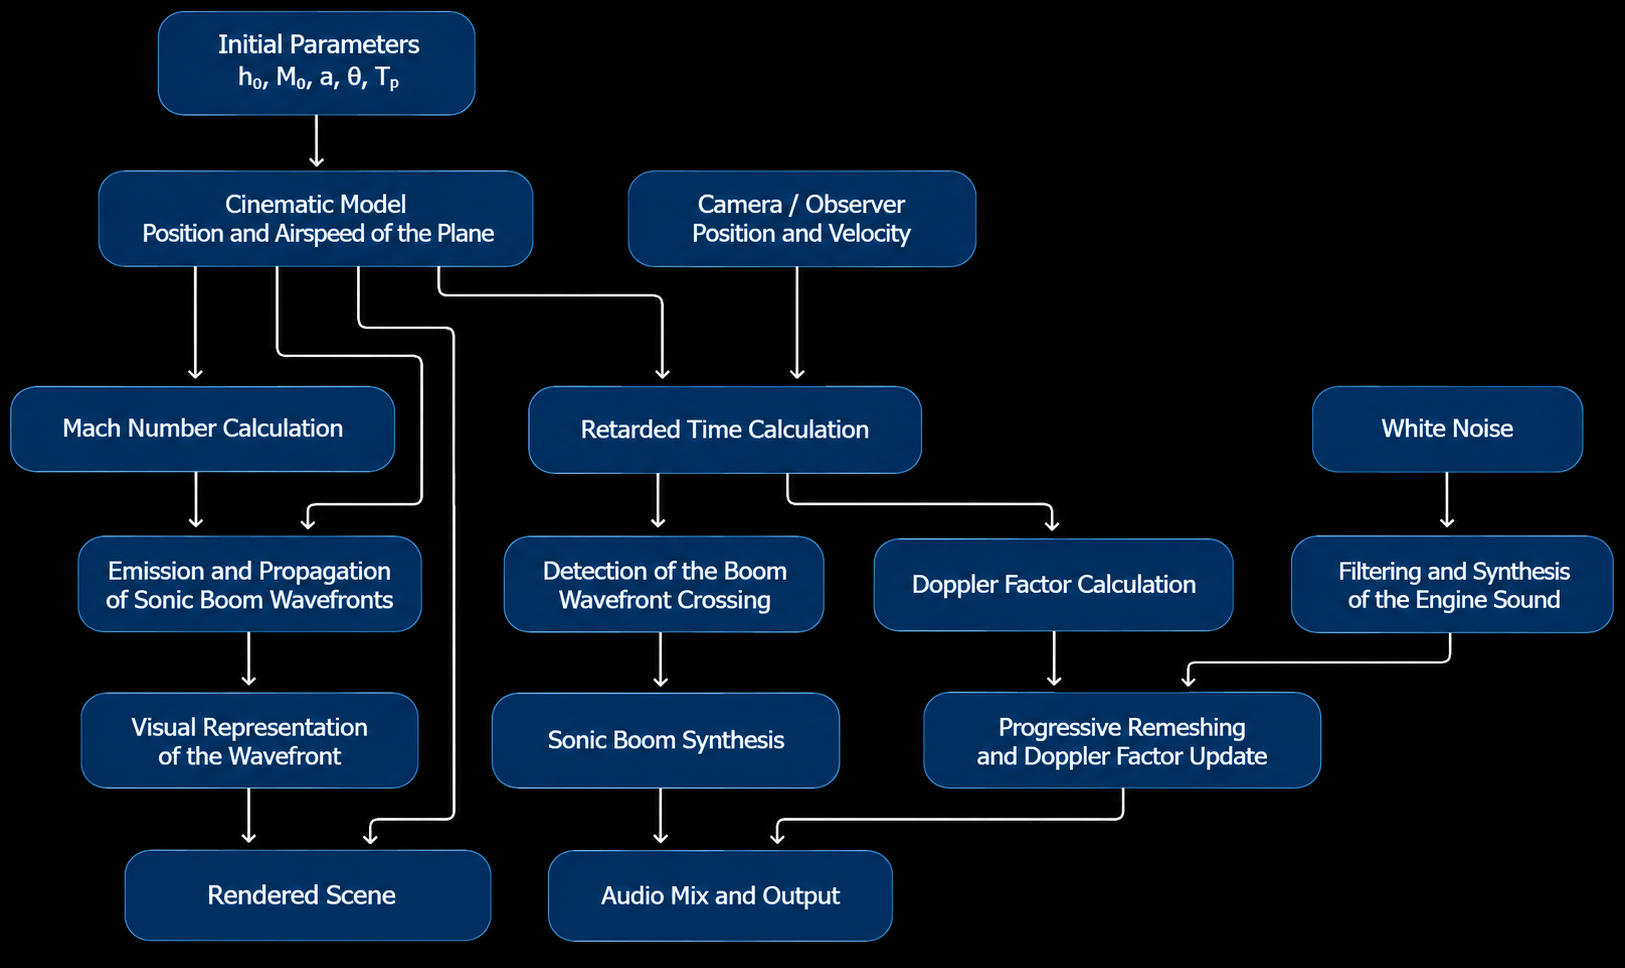
\includegraphics[width=\textwidth]{imgs/diagram.png}
	\end{figure} 
	
	\subsection{Algorithms and Computational Methods.}
	
	\begin{table}[H]
		\centering
		\label{tab:algoritmos}
		\begin{tabular}{|l|p{4cm}|p{10cm}|}
			\hline
			\textbf{Area} & \textbf{Algorithm or method} & \textbf{Application in the project} \\
			\hline
			Kinematics &
			Analytical evaluation &
			Computation of the aircraft's position, velocity, and acceleration from the equations of motion. \\
			\hline
			Atmosphere &
			Atmospheric model &
			Determination of the temperature and local speed of sound as a function of altitude. \\
			\hline
			Waves &
			Huygens' principle &
			Generation of spherical wavefronts from the aircraft's previous positions. \\
			\hline
			Waves &
			Envelope computation &
			Representation of the envelope of the wavefronts and determination of the geometry of the Mach cone. \\
			\hline
			Acoustics &
			Retarded-time solution &
			Numerical solution of the propagation equation to determine the emission instant of a signal received by the observer. \\
			\hline
			Acoustics &
			Doppler effect &
			Computation of the perceived frequency shift from the relative motion between the aircraft and the observer. \\
			\hline
			DSP &
			Noise synthesis &
			Generation of white-noise signals and spectral filtering to build the engine sound. \\
			\hline
			DSP &
			Variable resampling &
			Modification of the signal's playback rate to implement the Doppler shift. \\
			\hline
			DSP &
			Sonic boom synthesis &
			Generation of an N-type pressure signal associated with the arrival of the shock wave at the observer. \\
			\hline
			Graphics &
			Shader-based rendering &
			Rendering of the aircraft, wavefront geometry, and visual effects using OpenGL. \\
			\hline
			Real time &
			Discrete simulation loop &
			Independent updating of the physics, rendering, and audio processing. \\
			\hline
		\end{tabular}
	\end{table}
	
	\subsection{Dependencies and Libraries.}
	
	\begin{table}[H]
		\centering
		\label{tab:dependencias}
		\begin{tabular}{|l|l|p{10cm}|}
			\hline
			\textbf{Library} & \textbf{Module} & \textbf{Role in the project} \\ 
			\hline
			NumPy & \texttt{numpy} &
			Vector and matrix operations, array handling, and numerical computation. \\
			\hline
			SciPy & \texttt{scipy.signal} &
			Design and application of digital filters, signal processing, and interpolation operations. \\
			\hline
			SciPy & \texttt{scipy.optimize} &
			Numerical solution of nonlinear equations, especially for the retarded-time computation. \\
			\hline
			ModernGL & \texttt{moderngl} &
			Graphics rendering via OpenGL, shader management, and rendering of geometry and wavefronts. \\
			\hline
			SoundDevice & \texttt{sounddevice} &
			Real-time audio playback and generation through output devices. \\
			\hline
			SoundFile & \texttt{soundfile} &
			Reading and writing audio files, mainly in WAV format. \\
			\hline
			Matplotlib & \texttt{matplotlib} &
			Plotting of results, signal analysis, and validation of the models. \\
			\hline
			Librosa & \texttt{librosa} &
			Audio signal analysis, time--frequency representation, and extraction of spectral features. \\
			\hline
			Pytest & \texttt{pytest} &
			Automated unit testing to verify that the various modules work correctly. \\
			\hline
		\end{tabular}
	\end{table}
	
	\subsection{Testing and System Validation.}
	
	\begin{table}[H]
		\centering
		\label{tab:tests}
		\begin{tabular}{|l|p{4cm}|p{10cm}|}
			\hline
			\textbf{Area} & \textbf{Test} & \textbf{Validation criterion} \\
			\hline
			Kinematics &
			Trajectory validation &
			Comparison of the computed position and velocity with the analytical solutions of the motion model. \\
			\hline
			Atmosphere &
			Speed-of-sound validation &
			Checking the consistency of the temperature and speed of sound obtained for different altitudes. \\
			\hline
			Waves &
			Mach angle validation &
			Comparison of the geometry of the wavefront envelope with the theoretical relation $\sin(\mu)=1/M$. \\
			\hline
			Acoustics &
			Retarded-time validation &
			Checking the residual of the propagation equation and the temporal consistency of the solutions obtained. \\
			\hline
			Acoustics &
			Doppler effect validation &
			Comparison of the synthesized frequency with the theoretical frequency for different relative motions between source and observer. \\
			\hline
			DSP &
			Resampling validation &
			Checking the frequency shift using test signals of known frequency. \\
			\hline
			DSP &
			Continuity between audio blocks &
			Detection of discontinuities in the samples generated at the transitions between consecutive blocks. \\
			\hline
			DSP &
			Sonic boom validation &
			Checking that the acoustic event is generated when the shock front reaches the observer's position. \\
			\hline
			Graphics &
			Rendering validation &
			Checking the correspondence between the geometry computed by the physical model and its graphical representation. \\
			\hline
			System &
			Real-time performance &
			Measurement of frame rate, CPU load, and audio playback stability. \\
			\hline
			System &
			Numerical convergence &
			Comparison of results as the time step and the interval between wavefront emissions are reduced. \\
			\hline
		\end{tabular}
	\end{table}
	
	\subsection{Project Structure.}
	
	\begin{table}[H]
		\centering
		\label{tab:estructura}
		\begin{tabular}{|l|p{4cm}|p{10cm}|}
			\hline
			\textbf{Directory} & \textbf{Module} & \textbf{Responsibility} \\
			\hline
			\texttt{physics/} &
			\texttt{trajectory.py} &
			Computation of the aircraft's position, velocity, and acceleration. \\
			\cline{2-3}
			&
			\texttt{atmosphere.py} &
			Atmospheric model and computation of the local speed of sound. \\
			\cline{2-3}
			&
			\texttt{wavefronts.py} &
			Generation and updating of the wavefronts. \\
			\hline
			\texttt{acoustics/} &
			\texttt{retarded\_time.py} &
			Solution for the emission time corresponding to each reception instant. \\
			\cline{2-3}
			&
			\texttt{doppler.py} &
			Computation of the frequency shift due to relative motion. \\
			\cline{2-3}
			&
			\texttt{sonic\_boom.py} &
			Detection of the shock wave's arrival and generation of the acoustic event. \\
			\hline
			\texttt{dsp/} &
			\texttt{noise.py} &
			Generation of the noise signals used for sound synthesis. \\
			\cline{2-3}
			&
			\texttt{filters.py} &
			Design and application of digital filters. \\
			\cline{2-3}
			&
			\texttt{resampling.py} &
			Resampling of signals with a variable frequency ratio. \\
			\cline{2-3}
			&
			\texttt{audio\_engine.py} &
			Management of the audio stream and real-time playback. \\
			\hline
			\texttt{visualization/} &
			\texttt{renderer.py} &
			Management of the OpenGL context and rendering via ModernGL. \\
			\cline{2-3}
			&
			\texttt{shaders/} &
			GLSL programs for vertex and fragment processing. \\
			\cline{2-3}
			&
			\texttt{camera.py} &
			Management of the camera and of spatial transformations. \\
			\hline
			\texttt{analysis/} &
			\texttt{spectral\_analysis.py} &
			Spectral analysis and visualization of the generated signals. \\
			\cline{2-3}
			&
			\texttt{convergence.py} &
			Evaluation of the numerical convergence of the model. \\
			\cline{2-3}
			&
			\texttt{benchmarks.py} &
			Measurement of computational performance. \\
			\hline
			\texttt{tests/} &
			\texttt{test\_*.py} &
			Unit and integration tests for the various modules. \\
			\hline
			Root directory &
			\texttt{main.py} &
			Initialization and coordination of the simulation subsystems. \\
			\cline{2-3}
			&
			\texttt{requirements.txt} &
			Declaration of the project's external dependencies. \\
			\hline
		\end{tabular}
		
	\end{table}
	
	\newpage
	\begin{verbatim}
		concorde_simulation/
		|
		|-- main.py
		|-- requirements.txt
		|
		|-- physics/
		|   |-- trajectory.py
		|   |-- atmosphere.py
		|   |-- wavefronts.py
		|
		|-- acoustics/
		|   |-- retarded_time.py
		|   |-- doppler.py
		|   |-- sonic_boom.py
		|
		|-- dsp/
		|   |-- noise.py
		|   |-- filters.py
		|   |-- resampling.py
		|   |-- audio_engine.py
		|
		|-- visualization/
		|   |-- renderer.py
		|   |-- camera.py
		|   |-- shaders/
		|
		|-- analysis/
		|   |-- spectral_analysis.py
		|   |-- convergence.py
		|   |-- benchmarks.py
		|
		|-- tests/
		|   |-- test_trajectory.py
		|   |-- test_doppler.py
		|   |-- test_wavefronts.py
		|   |-- test_audio.py
	\end{verbatim}
	
	\newpage 
	
	\section{Task Schedule through February.}
	
	The project will be carried out in several stages between November 2026 and February 2027. The schedule provides for the progressive implementation of the different subsystems, starting with the physical model and continuing with the acoustic modules, digital signal processing, and graphical rendering. Finally, the components will be integrated, the results validated, and the technical documentation written.
	
	Tasks will be organized modularly, so that each subsystem can be developed and verified independently before being integrated into the main application.
	
	\begin{table}[H]
		\centering
		\label{tab:planificacion}
		\small
		\begin{tabular}{|c|p{3.1cm}|c|p{2.5cm}|p{2.5cm}|p{2.5cm}|}
			\hline
			\textbf{ID} & \textbf{Task} & \textbf{Duration} &
			\textbf{Owner} & \textbf{Dependencies} &
			\textbf{Milestone} \\
			\hline
			T1 & Environment setup and project architecture &
			1 week & Lead developer & None &
			Initial structure operational \\
			\hline
			T2 & Implementation and validation of the kinematic and atmospheric model &
			2 weeks & Lead developer & T1 &
			Functional physical model \\
			\hline
			T3 & Generation of wavefronts and Mach envelope &
			2 weeks & Lead developer & T2 &
			Validated geometric model \\
			\hline
			T4 & Implementation of retarded time and acoustic propagation &
			3 weeks & Lead developer & T2, T3 &
			Operational propagation model \\
			\hline
			T5 & Implementation of the Doppler effect and sonic boom synthesis &
			2 weeks & Lead developer & T4 &
			Complete acoustic model \\
			\hline
			T6 & Development of the audio engine and DSP processing &
			3 weeks & Lead developer & T5 &
			Real-time audio generation \\
			\hline
			T7 & Development of the renderer using ModernGL and shaders &
			3 weeks & Lead developer & T3 &
			Functional graphical representation \\
			\hline
			T8 & Integration of the physical, graphical, and acoustic subsystems &
			2 weeks & Lead developer & T5, T6, T7 &
			First integrated version \\
			\hline
			T9 & Testing, numerical validation, and optimization &
			2 weeks & Lead developer & T8 &
			Validated stable version \\
			\hline
			T10 & Documentation, results, and final report &
			2 weeks & Lead developer & T9 &
			Final delivery \\
			\hline
		\end{tabular}
	\end{table}
	
	\newpage
	
	\section{References.}
	
	\bibliographystyle{plain} 
	\bibliography{references}
	
\end{document}